% Simulations
\chapter{Anomaly Response Simulations}  \label{sec:numerical}
\section{State Feedback}
The two cases discussed above, of the introduction of actuator dynamics and a time delay, respectively, were simulated numerically in MATLAB/Simulink for bank angle tracking tasks. In these simulations, the commanded stability axis bank angle is a sequence of 5-second steps. In both of the examples presented here, the anomaly occurs at $t_{s,p} = 30$s, and the corrective action is applied to the controller at $t_{s,c} = 90$s.

Numerical data for the Boeing 747 flying straight-and-level at Mach 0.25 at sea level\cite{heffley1972aircraft} was substituted into (\ref{eqn:2nd_order_lateral}) to constitute the following nominal plant dynamics, beginning at time $t = 0$
\begin{equation}
		\dot{x}_p = \begin{bmatrix}
			0 & \hfil 1 \\ 0 & -1.10
		\end{bmatrix} x_p + \begin{bmatrix}
			0 \\ 0.318
		\end{bmatrix} \delta_a
\end{equation} \noindent which resulted in the open-loop transfer function 
\begin{equation}
		\frac{\Phi(s)}{\Delta_a(s)} = \frac{0.318}{s^2 + 1.10s}
\end{equation}

A reference model was chosen as in (\ref{eqn:rm_2_symbolic}) given by
\begin{equation}
	\dot{x}_m = \underbrace{\begin{bmatrix}
		\hfil 0 & \hfil 1\\ -8 & -6
	\end{bmatrix}}_{A_m} x_m + \underbrace{\begin{bmatrix}
		0 \\ 8
	\end{bmatrix}}_{B_m} r - \underbrace{\begin{bmatrix}
		\hfil -10 & \hfil -1 \\ \hfil 8 & \hfil -4
	\end{bmatrix}}_{L_m} e
	\label{eqn:rm_2}
\end{equation}
\noindent for the first (``nominal'' and ``post-anomaly'') stages of simulation. The initial feedback and feedforward parameters $\theta(t=0)$ and $q(t=0)$ are chosen such that the matching conditions of (\ref{e:tstar}) and (\ref{e:qstar}) are met.

% TODO fix step response plots with x-axis label cut off
\subsection{Actuator Fault}
By applying the change in dynamics defined in (\ref{eqn:actuator_dynamics_symbolic}), and choosing $T_l = 0.556$, the plant dynamics in (\ref{eqn:plant_3_symbolic}) become
\begin{equation}
	\dot{x}_p' = \begin{bmatrix}
		0 & \hfil 1 & \hfil 0\\ 0 & \hfil 0 & \hfil 1 \\ 0 & -1.98 & -2.90
	\end{bmatrix} x_p' + \begin{bmatrix}
		0 \\ 0 \\ 0.5724
	\end{bmatrix} u
	\label{eqn:plant_3}
\end{equation}
\noindent at $t = t_{s,p}$, resulting in the open-loop transfer function
\begin{equation}
		\frac{\Phi(s)}{U(s)} = \frac{0.5724}{s^3 + 2.90s^2 + 1.98s}\\
\end{equation}

After detection and diagnosis of the anomaly with the shared decision-making framework, the corrective action to increase the dimension of the controller is made at $t = t_{s,c}$, and the reference model dynamics (with a pole added to the second-order reference model at $s = -4$) becomes that of (\ref{eqn:rm_3_symbolic}) given by
\begin{equation}
	\dot{x}_m' = \underbrace{\begin{bmatrix}
		\hfil 0 & \hfil 1 & \hfil 0\\ \hfil 0 & \hfil 0 & \hfil 1 \\ -32 & -32 & -10
	\end{bmatrix}}_{A_m'} x_m' + \underbrace{\begin{bmatrix}
		0 \\ 0 \\ 32
	\end{bmatrix}}_{B_m'} r - \underbrace{\begin{bmatrix}
		-10 & -1 & \hfil 0 \\ \hfil 0 & -10 & -1 \\ \hfil 32 & \hfil 32 & \hfil 0
	\end{bmatrix}}_{L_m'} e'
	\label{eqn:rm_3}
\end{equation}

The feedback (and corresponding feedforward) gains which will cause the closed-loop roll response to match the desired response exactly are
\begin{align}
	\theta^*(t) = & \begin{cases}
		\begin{bmatrix}
			-25.16, & -15.41
		\end{bmatrix}  & t < t_{s,p} \\
		\begin{bmatrix}
			-55.91, & -52.45, & -5.07
		\end{bmatrix} & t \geq t_{s,p}
	\end{cases} \\
	q^*(t) = & \begin{cases}
		25.16 & t < t_{s,p} \\
		55.91 & t \geq t_{s,p}
	\end{cases}
\end{align}
\noindent which are unknown to the adaptive controller. As mentioned earlier, we chose $\theta(t=0)= [-25.16, \quad -15.41]$ and $q(t=0)=25.16$. The learning rates in (\ref{eqn:thetadot_projection}) and (\ref{eqn:qdot_projection}) were chosen to be $\Gamma_\theta = 10 I_2$, with $I_n$ the identity matrix of dimension $n$, and $\gamma_q = 10$. The projection operator was not used in this simulation. It was assumed that $t_{s,p}=30$s and $t_{s,c}=90$s. To add more realism to the simulation example, we have assumed that the signal $\dot{p}$ is not directly measured, and instead use a high-pass filter to estimate it from $p$ using $\hat{\dot{p}} = \frac{as}{s+a} p$. Results of this simulation are given in Figures \ref{fig:command_and_output}, \ref{fig:theta}, \ref{fig:error}, and \ref{fig:step_pole}. 

\begin{figure}[h!]
	\centering
	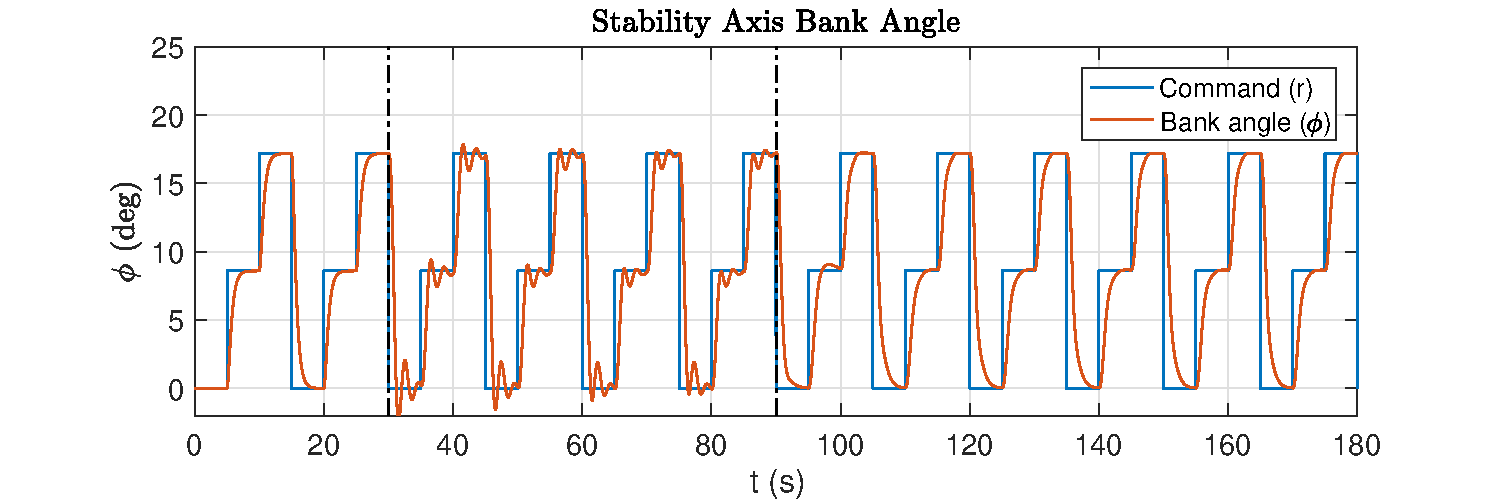
\includegraphics[width=\columnwidth]{phi_pole.pdf}
	\caption{Command ($r$) and output ($\phi$): under nominal operation ($t \leq 30$ s), after the change in actuator dynamics ($30$ s $< t \leq 90$ s), and after a corrective action to switch the controller ($t > 90$ s)}
	\label{fig:command_and_output}
\end{figure}

\begin{figure}[h!]
	\centering
	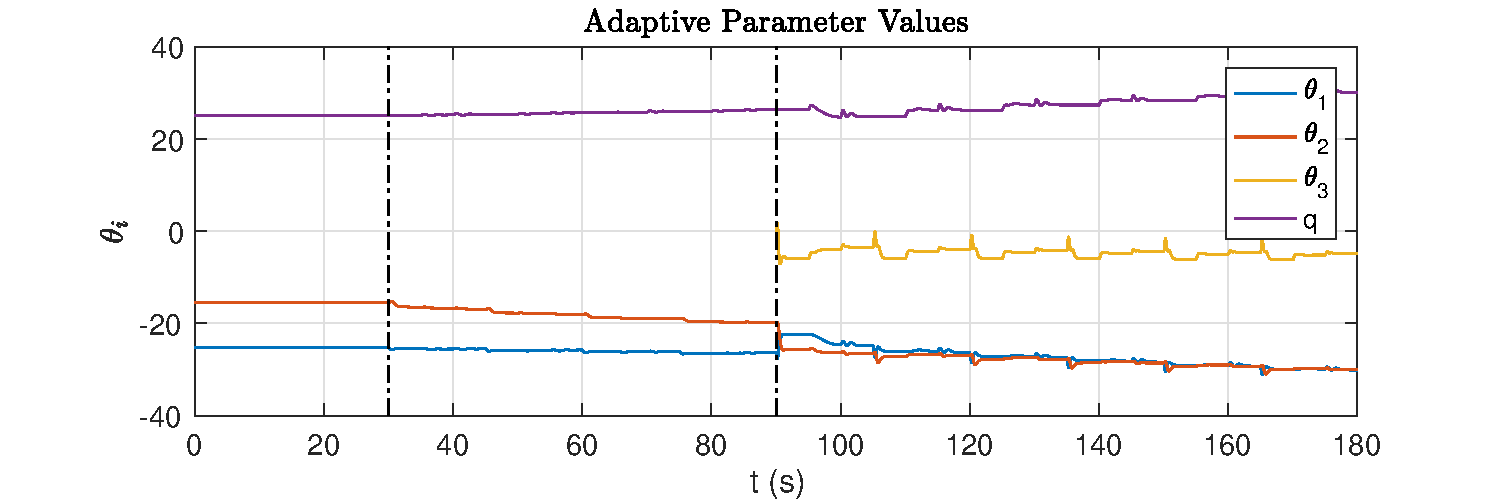
\includegraphics[width=\columnwidth]{theta_pole.pdf}
	\caption{Adaptive feedback gains for the same simulation example as in Figure \ref{fig:command_and_output}: under nominal operation ($t \leq 30$ s), after the change in actuator dynamics ($30$ s $< t \leq 90$ s), and after a corrective action to switch the controller ($t > 90$ s)}
	\label{fig:theta}
\end{figure}

\begin{figure}[h!]
	\centering
	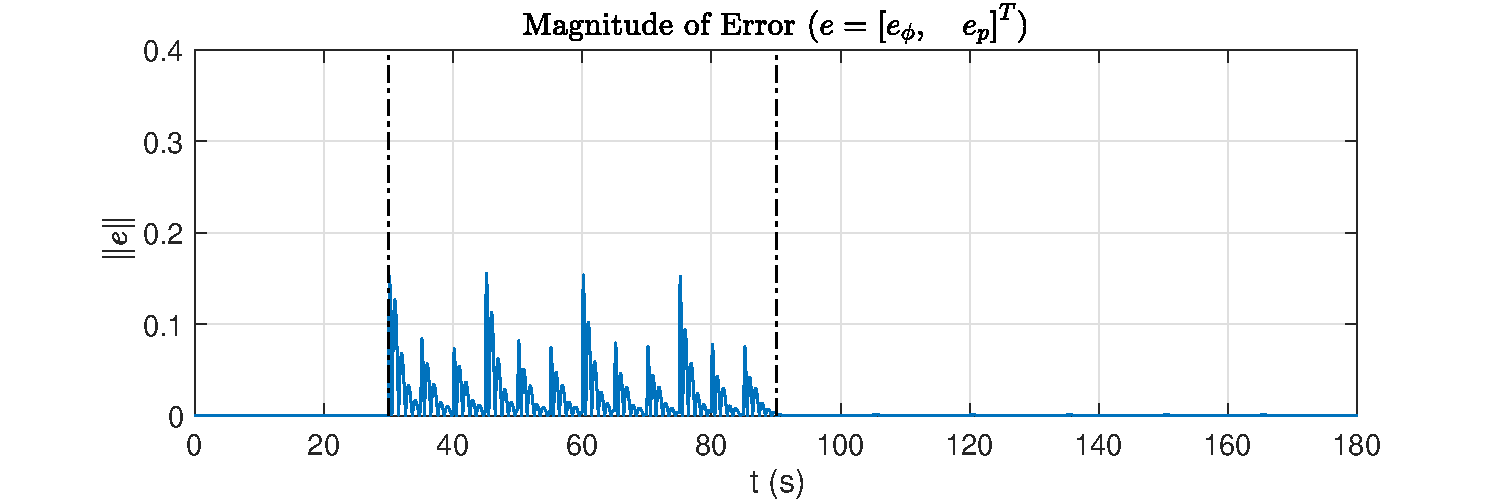
\includegraphics[width=\columnwidth]{e_pole.pdf}
	\caption{The tracking error $e$ for the same simulation example as in Figure \ref{fig:command_and_output}: under nominal operation ($t \leq 30$ s), after the change in actuator dynamics ($30$ s $< t \leq 90$ s), and after a corrective action to switch the controller ($t > 90$ s)}
	\label{fig:error}
\end{figure}

From Figures \ref{fig:command_and_output}, \ref{fig:theta}, and \ref{fig:error}, it is clear that after an initial adaptation period, the adaptive controller with third-order reference model dynamics converges on the desired feedback/feedforward gains, returning the roll control to its satisfactory performance without requiring any manual control from the human pilot. The action required from the human pilot is in the detection and diagnosis of the anomaly in dynamical behavior, leading to the addition of feedback on $\hat{\dot{p}}$ as a corrective action. 

Taking average parameter values over time $\Delta t$ at the end of each stage of simulation (Nominal, Post-Anomaly, Post-Correction)
\begin{align}
	\bar{\theta}_{t_i} &= \frac{1}{\Delta t} \int_{t_{f,i}-\Delta t}^{t_{f,i}} \theta(t) dt, \qquad i = [1, 2, 3] \label{eqn:theta_bar}\\
	\bar{q}_{t_i} &= \frac{1}{\Delta t} \int_{t_{f,i}-\Delta t}^{t_{f,i}} q(t) dt, \qquad i = [1, 2, 3] \label{eqn:q_bar}
\end{align}
with $\Delta t = 5$s, $t_f = [30, \quad 90, \quad 180]$ allows us to define a closed-loop frequency response which is representative of controller performance after parameter adaptation in each stage. Figure \ref{fig:step_pole} shows the closed-loop unit step input responses with $(\bar{\theta}_i, \bar{q}_i)$ for $i = [1, 2, 3]$ plotted alongside the ideal response during nominal operation, demonstrating how the characteristics of nominal operation are recovered with the adaptive controller with three feedback parameters.

\begin{figure}[h!]
	\centering
	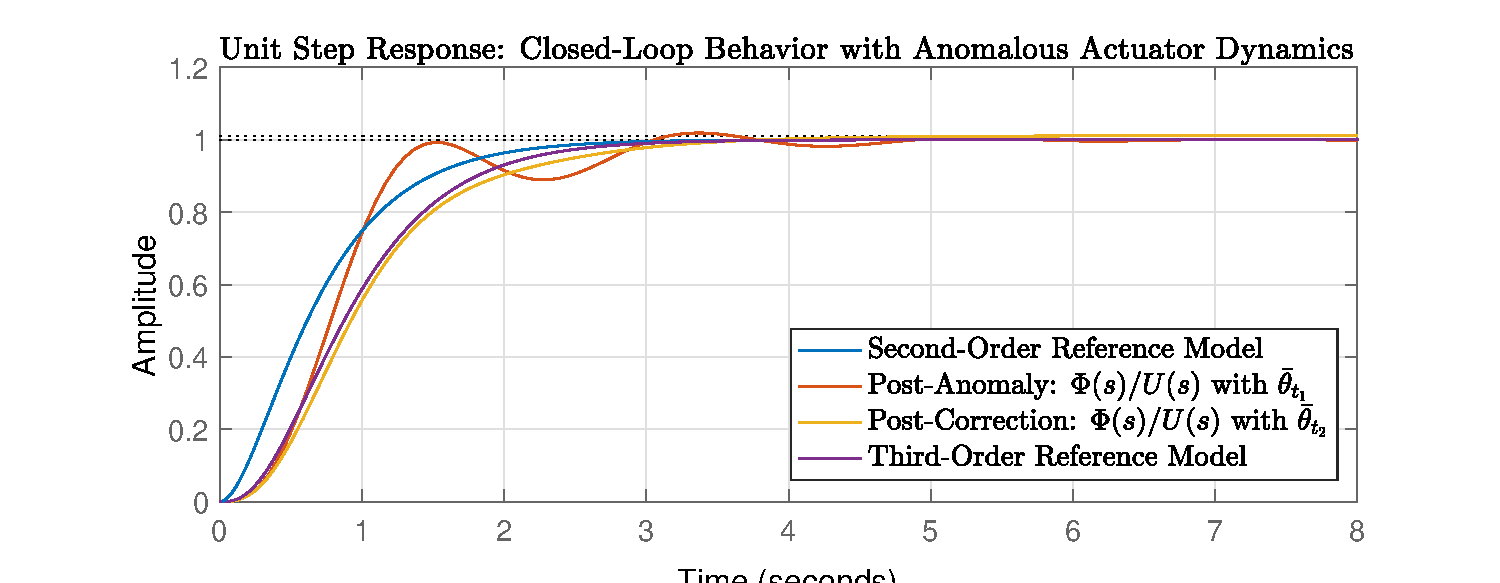
\includegraphics[width=\columnwidth]{step_pole.pdf}
	\caption{Unit step responses for closed-loop transfer functions at different stages of simulation in case (i), demonstrating performance improvement after corrective action}
	\label{fig:step_pole}
\end{figure}

\subsection{Time-Delayed Sensor Measurements}
A time delay of $\tau = 0.200$s is added to the plant (\ref{eqn:2nd_order_lateral}) between the state measurements and their use in control input computation. The reference models given by (\ref{eqn:rm_2}) and 
\begin{equation}
	\dot{x}_m' = \underbrace{\begin{bmatrix}
		\hfil 0 & \hfil 1 & \hfil 0\\ \hfil 0 & \hfil 0 & \hfil 1 \\ -32 & -32 & -10
	\end{bmatrix}}_{A_m'} x_m' + \underbrace{\begin{bmatrix}
		0 \\ 0 \\ 32
	\end{bmatrix}}_{B_m'} r - \underbrace{\begin{bmatrix}
		-10 & -1 & \hfil 0 \\ \hfil 0 & \hfil -10 & \hfil -1 \\ \hfil 32 & \hfil 32 & \hfil 9.9
	\end{bmatrix}}_{L_m'} e'
	\label{eqn:rm_3_delay}
\end{equation}
\noindent are used in the Nominal and Post-Correction intervals, respectively. With $\Phi_\sigma(s)$ defined as the delayed bank angle measurement, the change in the transfer function $\Phi_\sigma(s)/U(s)$ is thus
\begin{equation}
		\frac{\Phi_\sigma(s)}{U(s)} = \begin{cases}
			\frac{0.318}{s^2 + 1.10s} & t < t_{s,p}\\
			\frac{0.318}{s^2 + 1.10s}e^{-0.20 s} & t \geq t_{s,p}
		\end{cases} 
\end{equation}

Using the first-order delay approximation (\ref{first_order_delay_approx}), so that $e^{-0.20 s}$ is approximated as $1/(1+0.20s)$, the feedback and feedforward gains which would give the desired closed-loop response for $\Phi_\sigma(s)/U(s)$ are
\begin{align}
	\theta^*(t) = & \begin{cases} \begin{bmatrix} -25.16, & -15.41 \end{bmatrix} & t < t_{s,p} \\ \begin{bmatrix}-20.13, & -16.67, & -2.45\end{bmatrix} & t \geq t_{s,p} \end{cases} \\
	q^*(t) = &\begin{cases} 25.16 & t < t_{s,p} \\ 20.13 & t \geq t_{s,p} \end{cases}
\end{align}

\noindent The learning rates chosen for this simulation were
\begin{align}
	\Gamma_\theta  = & \begin{cases}
		10 I_2 & t < t_{s,c}\\
		\text{diag}(10.0, 10.0, 0.1) & t \geq t_{s,c}
 	\end{cases} \\
	\gamma_q  = &\quad 10.0 \qquad ~ \qquad ~ \qquad ~ \quad \forall t
\end{align}

\noindent where the learning rate on $\hat{\dot{p}}$ is lower than that used in the simulation of case (i). This lower learning rate was needed as the approximation of the time delay as a first-order lag is fairly restrictive. In addition, a projection operator with the following constant parameters (\ref{eqn:proj_function}) was used to limit $\dot{\theta}(t)$
\begin{align}
	\varphi_m = & \begin{bmatrix}
		300, & 200, & 25
	\end{bmatrix} \\
	\varphi_{\epsilon} = & \begin{bmatrix}
		50, & 50, & 25
	\end{bmatrix}\end{align}
\noindent and the following constant parameters for the projection operator limiting $\dot{q}(t)$
\begin{align}
	\varphi_m = &~ 300\\
	\varphi_{\epsilon} = &~ 50
\end{align}

\begin{figure}[h!]
	\centering
	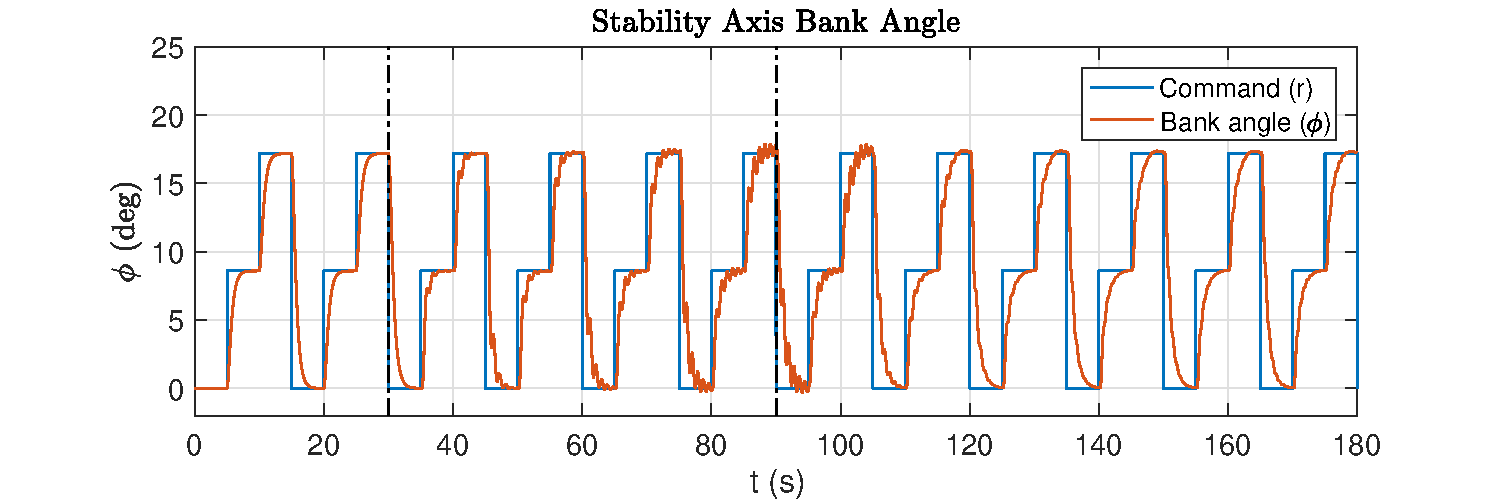
\includegraphics[width=\columnwidth]{phi_delay.pdf}
	\caption{Command ($r$) and output ($\phi$): under nominal operation ($t \leq 30$ s), after the sudden addition of a time delay ($30$ s $< t \leq 90$ s), and after a corrective action to switch the controller ($t > 90$ s)}
	\label{fig:command_and_output_d}
\end{figure}

\begin{figure}[h!]
	\centering
	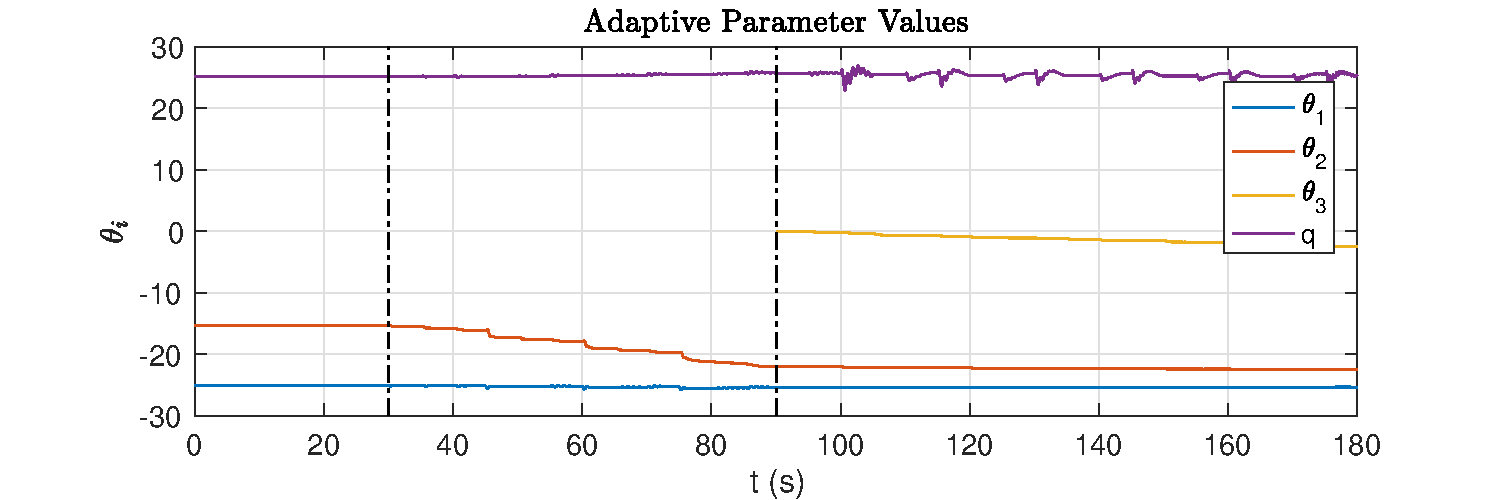
\includegraphics[width=\columnwidth]{theta_delay.pdf}
	\caption{Adaptive feedback gains for the same simulation example as in Figure \ref{fig:command_and_output_d}: under nominal operation ($t \leq 30$ s), after the sudden addition of a time delay ($30$ s $< t \leq 90$ s), and after a corrective action to switch the controller ($t > 90$ s)}
	\label{fig:theta_d}
\end{figure}

\begin{figure}[h!]
	\centering
	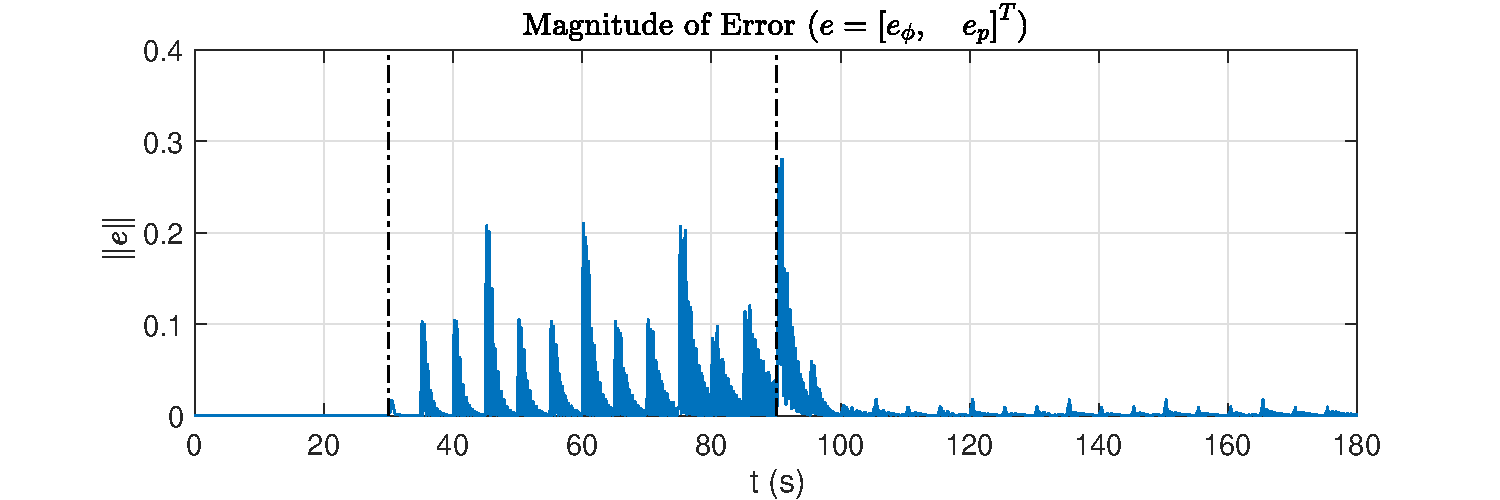
\includegraphics[width=\columnwidth]{e_delay.pdf}
	\caption{The tracking error $e$ for the same simulation example as in Figure \ref{fig:command_and_output_d}: under nominal operation ($t \leq 30$ s), after the sudden addition of a time delay ($30$ s $< t \leq 90$ s), and after a corrective action to switch the controller ($t > 90$ s)}
	\label{fig:error_d}
\end{figure}

The resulting responses of the shared controller are shown in Figures \ref{fig:command_and_output_d}, \ref{fig:theta_d}, and \ref{fig:error_d}. From these results, we see that the MRAC controller with two feedback parameters has trouble tracking the commanded bank angle after the introduction of an anomaly, but the addition of a third feedback parameter ($\hat{\dot{p}}$) and a corresponding increase in the dimension of the reference model allows the controller to recover a reasonable tracking performance. It is worth noting that the model-following error does not converge to zero even with the MRAC controller given by (\ref{eqn:control_law}), (\ref{eqn:thetadot_projection}), (\ref{eqn:qdot_projection}), and (\ref{eqn:rm_3}), because of the time delay approximation. 

The transfer functions used to generate step response plots in Figure \ref{fig:step_delay} use (\ref{eqn:theta_bar}) and (\ref{eqn:q_bar}) for average parameter values. Although the step response characteristics of Post-Correction differ more from nominal operation compared to case (i), the closed-loop response of Post-Correction is significantly more satisfactory than Post-Anomaly.

\begin{figure}[h!]
	\centering
	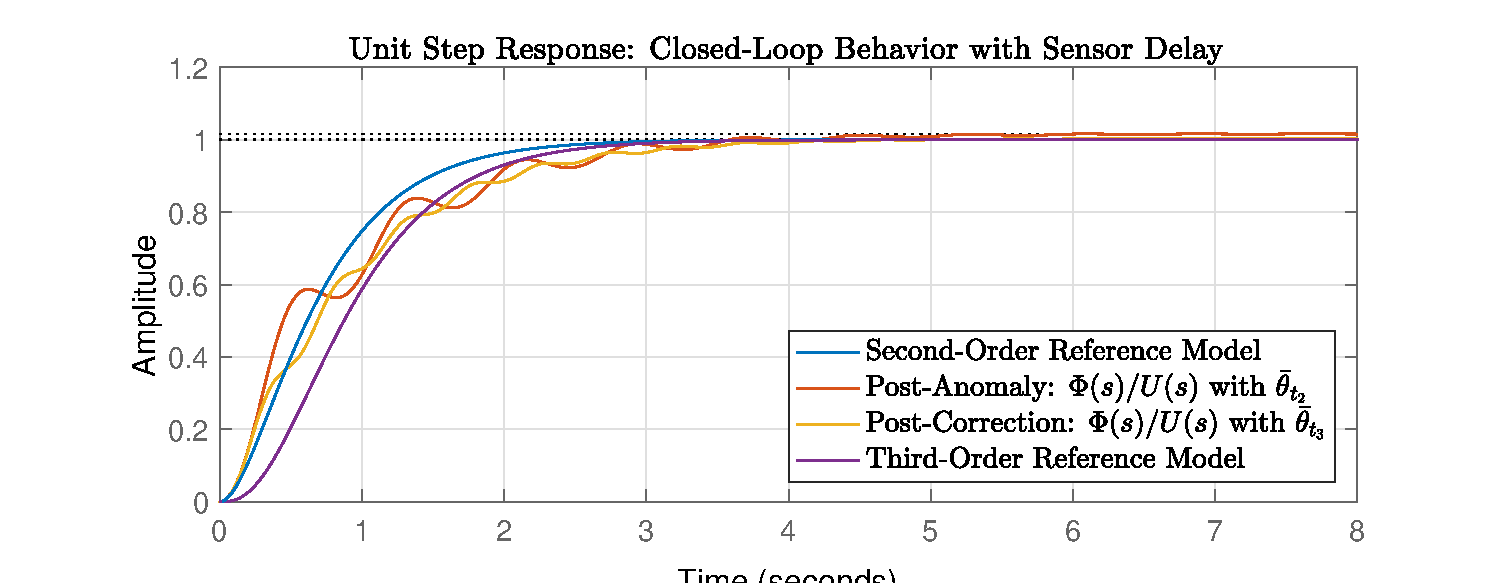
\includegraphics[width=\columnwidth]{step_delay.pdf}
	\caption{Unit step responses for closed-loop transfer functions at different stages of simulation in case (ii), demonstrating performance improvement after corrective action}
	\label{fig:step_delay}
\end{figure}

The shared control solution introduced in Section \ref{sec:shared_ctrl} is applied to the problem introduced in Section \ref{sec:problem} on a high altitude, long endurance (HALE) very flexible aircraft (VFA) model. The aircraft model used in simulation, developed by \cite{gibson2011modeling} for longitudinal control design applications, is rendered in Figure \ref{fig:vfa} and described in Section \ref{subsec:vfa_model}. The results of numerical simulations on the control and anomaly recovery with this MIMO plant are then presented in Section \ref{subsec:sims}, comparing the shared anomaly response to alternative anomaly responses.

\section{Output Feedback}

\subsection{HALE Aircraft Model}\label{subsec:vfa_model}
%HALE VFA.
High altitude long endurance (HALE) aerial platforms, such as the solar-electric NASA/AeroVironment Helios and Facebook Aquila, have unique design considerations to satisfy goals of uninterrupted weeks- or months-long operation. To reduce power draw, HALE aircraft designs save mass by allowing wings to bend, and may be classified as very flexible aircraft (VFA). Compared to typical fixed-wing aircraft, these aircraft operate at low speed, and may use low-bandwidth actuators which must be accounted for in control design. HALE VFA platforms are likely to have significant modeling uncertainties and online variation in dynamics due to flexible effects and degradation over long-term operation. Although these platforms are unmanned aerial vehicles (UAVs), they require supervision from remote human operators.

\begin{figure}[htbp]
	\centering
	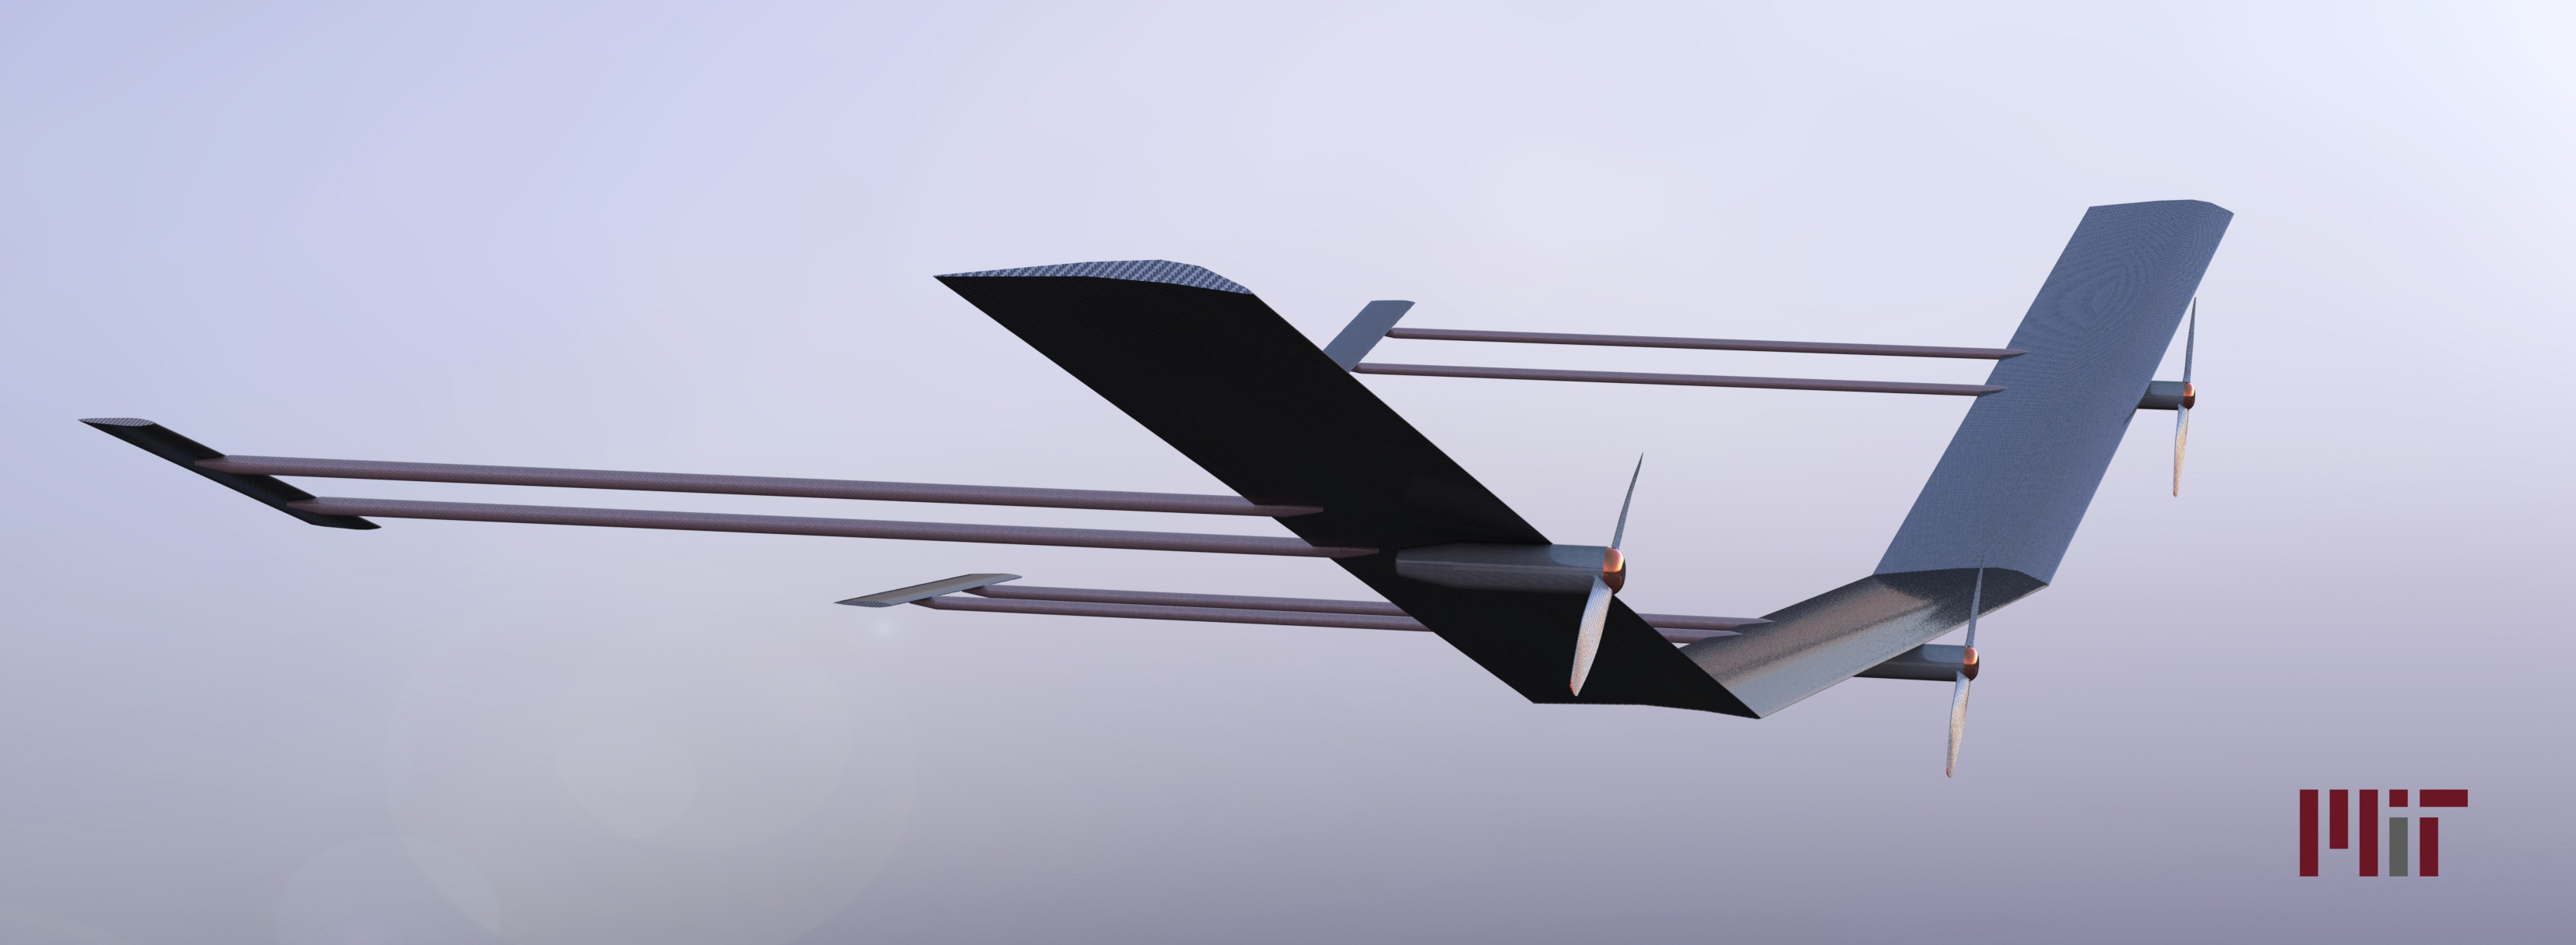
\includegraphics[width=0.95\columnwidth]{VFA_16.jpg}
	\caption{Rendering of very flexible aircraft model}
	\label{fig:vfa}
\end{figure}

The aircraft model used in simulation represents the nonlinear longitudinal dynamics of a HALE VFA concept with three rigid lifting sections, hinged together such that the aircraft is able to bend at the joints of the three sections. The pitch mode dynamics of this nonlinear model is defined by the state vector
\begin{equation}
x_{\text{vfa}} = \begin{bmatrix}
~V~\\
\alpha \\
h \\
\theta \\
q\\
\eta\\
\dot{\eta}
\end{bmatrix} =
\begin{bmatrix}
	 $Airspeed (ft/s)$\\ $Angle of attack (rad)$\\ $Altitude (ft)$\\ $Pitch angle (rad)$\\ $Pitch rate (rad/s)$\\ $Dihedral (rad)$\\ $Dihedral rate (rad/s)$
\end{bmatrix}
\end{equation}

We linearize and trim the aircraft in straight and level flight using the inputs
\begin{equation}
	u_{\text{vfa}} = \begin{bmatrix}
\delta_{th} \\
\delta_{a,c} \\
\delta_{a,o} \\
\delta_{e,c} \\
\delta_{e,o} 
\end{bmatrix} = \begin{bmatrix}
		$Thrust (lbf)$\\
		$Center aileron (rad)$\\
		$Outer aileron (rad)$\\
		$Center elevator (rad)$\\
		$Outer elevator (rad)$
	\end{bmatrix}
\end{equation}

Assuming small deviations in altitude, the state vector corresponding to (\ref{eq:plant_dynamics}) is
\begin{equation}
	x_p = \begin{bmatrix}
V & \; \alpha & \; \theta & \; q & \; \eta & \; \dot{\eta}
\end{bmatrix}^T.
\end{equation}

We consider the control task of tracking commands for the dihedral angle and vertical acceleration, using control inputs $\delta_{a,o}$ and $\delta_{e,c}$ only, so the vector $u_p$ in (\ref{eq:plant_dynamics}) is
\begin{equation}
	u_p = \begin{bmatrix}
\delta_{a,o} & \; \delta_{e,c}
\end{bmatrix}^T.
\end{equation}

Regulation of the dihedral angle is desired, as a large dihedral angle is inefficient for lift generation and introduces instability in the open-loop dynamics, while a small dihedral angle will require more control effort to hold, increasing drag and power requirements and imparting twisting moments on the aircraft. 

The measurements available for control design are the pitch rate, dihedral angle, and vertical acceleration, leading to plant outputs
\begin{equation}
\begin{aligned}
y_p =& \, \Big[\; q \; \Big] \;= \Big[\: \text{Pitch rate (rad/s)} \:\Big] \\
z_p =& \begin{bmatrix}
\eta \\
A_z
\end{bmatrix} =\begin{bmatrix}
	$Dihedral angle (rad)$\\
	$Vertical acceleration (ft/s)$
\end{bmatrix}		
\end{aligned}
\end{equation}
and the outputs for the augmented plant (\ref{eq:augmented_plant}),
\begin{equation}
y = \begin{bmatrix}
	q \\ \int{z_p - z_{cmd}}
\end{bmatrix}, \quad z = z_p.
\end{equation}

For numerical simulations, the VFA model is trimmed at an airspeed of $68$ ft/s, altitude of $40,000$ ft, $2.8^\circ$ angle of attack and pitch angle (level flight), and dihedral angles ranging from $0$ to $20^\circ$ in $1^\circ$ increments. Figure \ref{fig:trim-poles} shows pole locations of the linearized plant for different dihedral angles, and Figure \ref{fig:trim-poles-zoom} shows instability of the linearized plant when trimmed above $11^\circ$ dihedral. Figure \ref{fig:trim-inputs} shows the thrust and control surface deflections for the trimmed VFA model over a range of dihedral angles.

\begin{figure}[htbp]
	\centering
	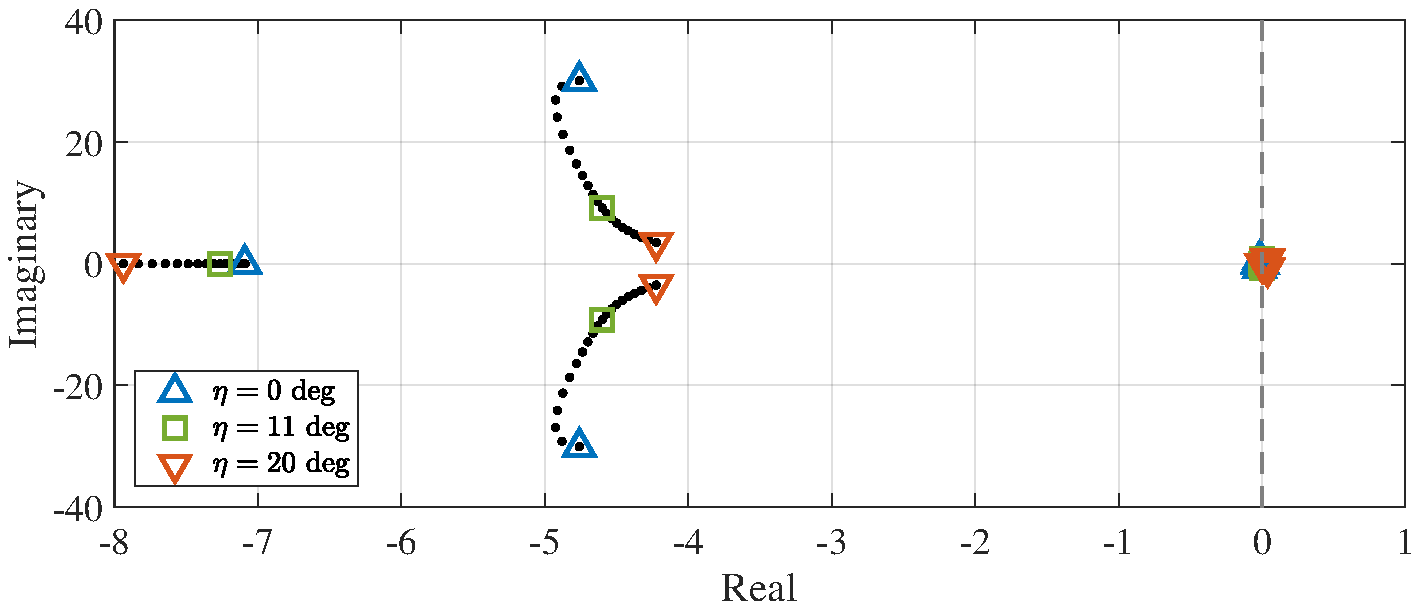
\includegraphics[width=0.95\columnwidth]{trim-poles-2.pdf}
	\caption{Poles of linearized system for different dihedral angles}
	\label{fig:trim-poles}
\end{figure}

\begin{figure}[htbp]
	\centering
	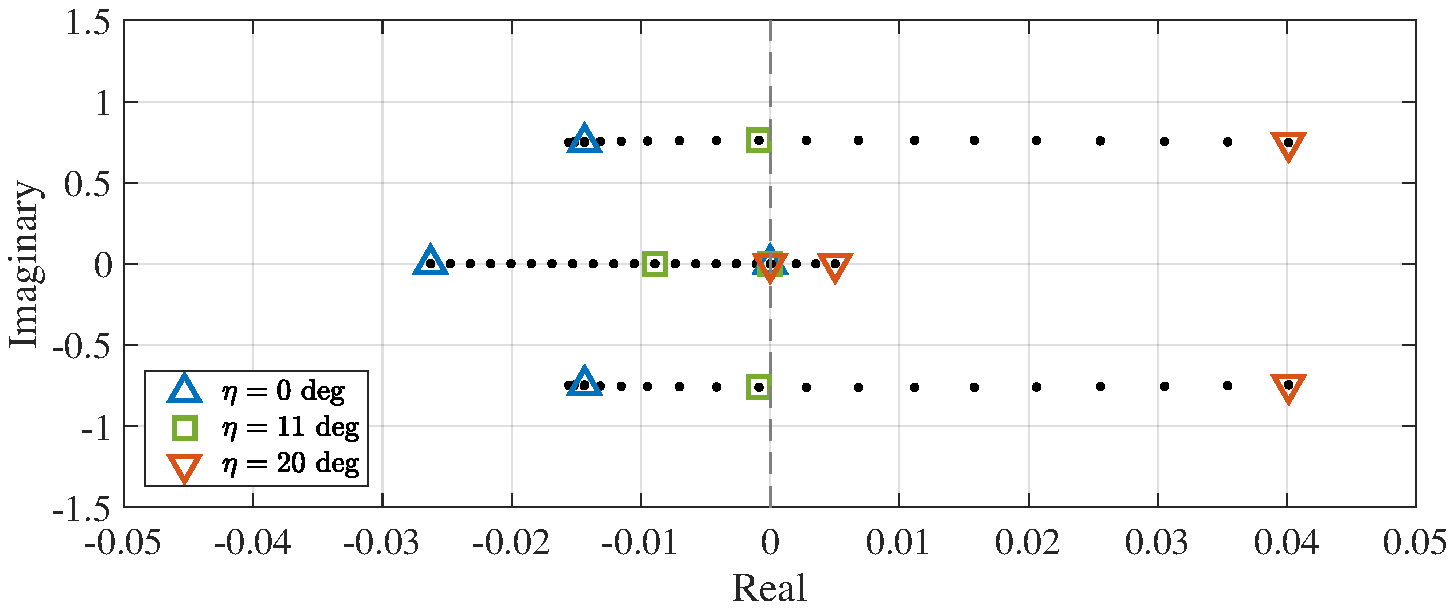
\includegraphics[width=0.95\columnwidth]{trim-poles-zoom-2.pdf}
	\caption{Dominant poles of linearized system, which move into the right-half complex plane when $\eta > 11^\circ$}
	\label{fig:trim-poles-zoom}
\end{figure}

\begin{figure}[htbp]
	\centering
	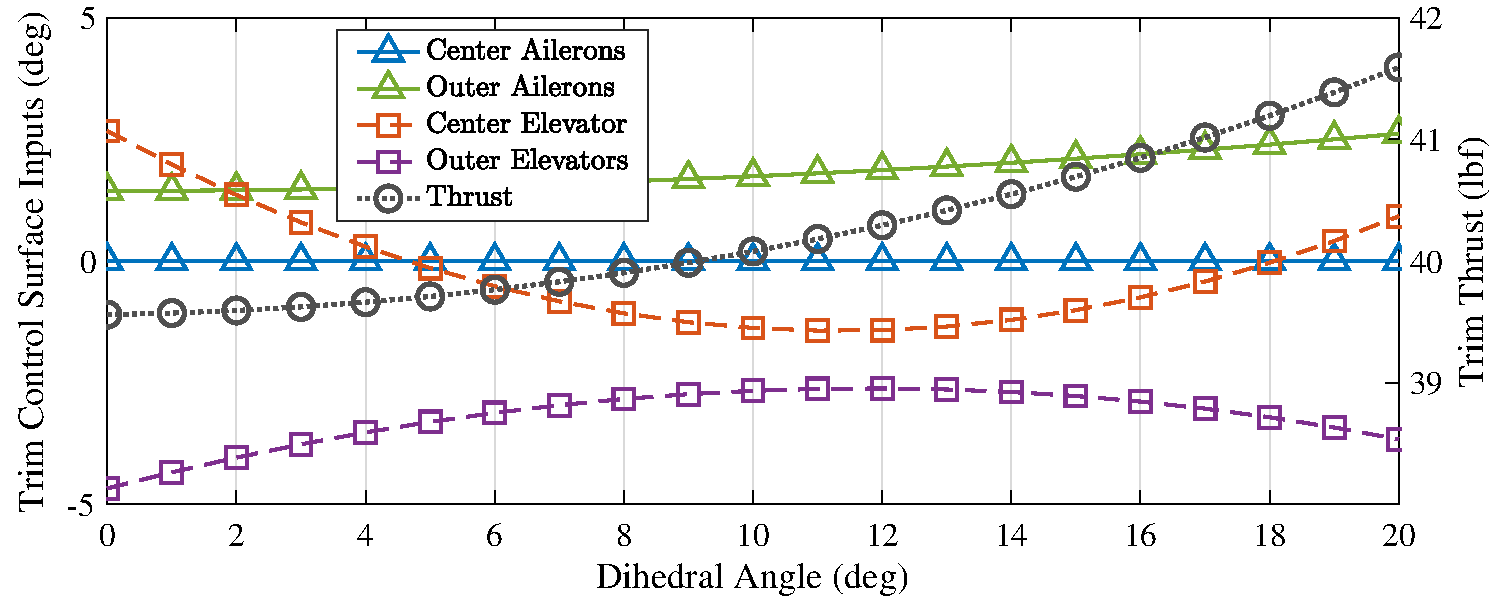
\includegraphics[width=0.95\columnwidth]{trim-inputs-3.pdf}
	\caption{Actuator trim at different dihedral angles}
	\label{fig:trim-inputs}
\end{figure}

The plant is augmented with a linear actuator model corresponding to (\ref{eq:first_order_act}) in the nominal case and (\ref{eq:second_order_act}) in the presence of anomalous dynamics. The vehicle simulation with first-order actuators (\ref{eq:first_order_act}) uses time constants $(\hat{\tau},\;\tau) = (0.5,\,2)$s in the control model and the actual plant, respectively, corresponding to
\begin{equation}
D_1 = 2 I_2, \quad \Theta_1 = -1.5 I_2
\end{equation}
where $\Theta_1$ is unknown for control design, and $I_2$ is the $2 \times 2$ identity matrix. 

Simulation of the anomalous dynamics (\ref{eq:second_order_act}) uses second-order actuators with cutoff frequencies $(\hat{\omega}_c,\; \omega_c) = (2 ,\; 1)$ rad/s and damping ratios $(\hat{\zeta},\; \zeta) = (0.7,\; 0.8)$ in the control model and actual plant, respectively, corresponding to
\begin{equation}
\begin{bmatrix}
	D_1 \\ D_2
\end{bmatrix} = \begin{bmatrix}
	4 I_2 \\ 2.8 I_2
\end{bmatrix}, \quad \begin{bmatrix}
	\Theta_1 \\ \Theta_2 
\end{bmatrix} = \begin{bmatrix}
	-3.75 I_2 \\ -2 I_2
\end{bmatrix}
\end{equation}
where $\Theta_1$ and $\Theta_2$ are unknown for control design. The uncertainty matrices $\Theta_p$ and $\Lambda$ are given by
\begin{equation}
\begin{gathered}
\Theta_{p}^{T}=\begin{bmatrix}
0.6 & -4.52 & \; 0 & \hfill 0.05 & \hfill 0.41 & \hfill 1.47\\
0.1 & \hfill 1.83 & \; 0 & -0.02 & -0.35 & -0.59
\end{bmatrix}\\ \Lambda = 0.2 I_2 \end{gathered}
\end{equation}
representing a poor linearization of the nonlinear model, and an 80\% reduction in actuator effectiveness.

\subsection{Numerical Simulations and Results} \label{subsec:sims}
We begin by simulating the HALE VFA under nominal autonomous control, responding to step inputs in commands for the dihedral angle and vertical acceleration, with the following three variants.
\begin{description}
	\item[Nom-1] Baseline RSLQR without uncertainty in control model
	\item[Nom-2] Baseline RSLQR with uncertainty in control model ($\Theta_p$, $\Lambda_p$, and $\Theta_1$)
	\item[Nom-3] Baseline RSLQR + MRAC with uncertainty in control model ($\Theta_p$, $\Lambda_p$, and $\Theta_1$)
\end{description}

\begin{figure}[htbp]
	\centering
	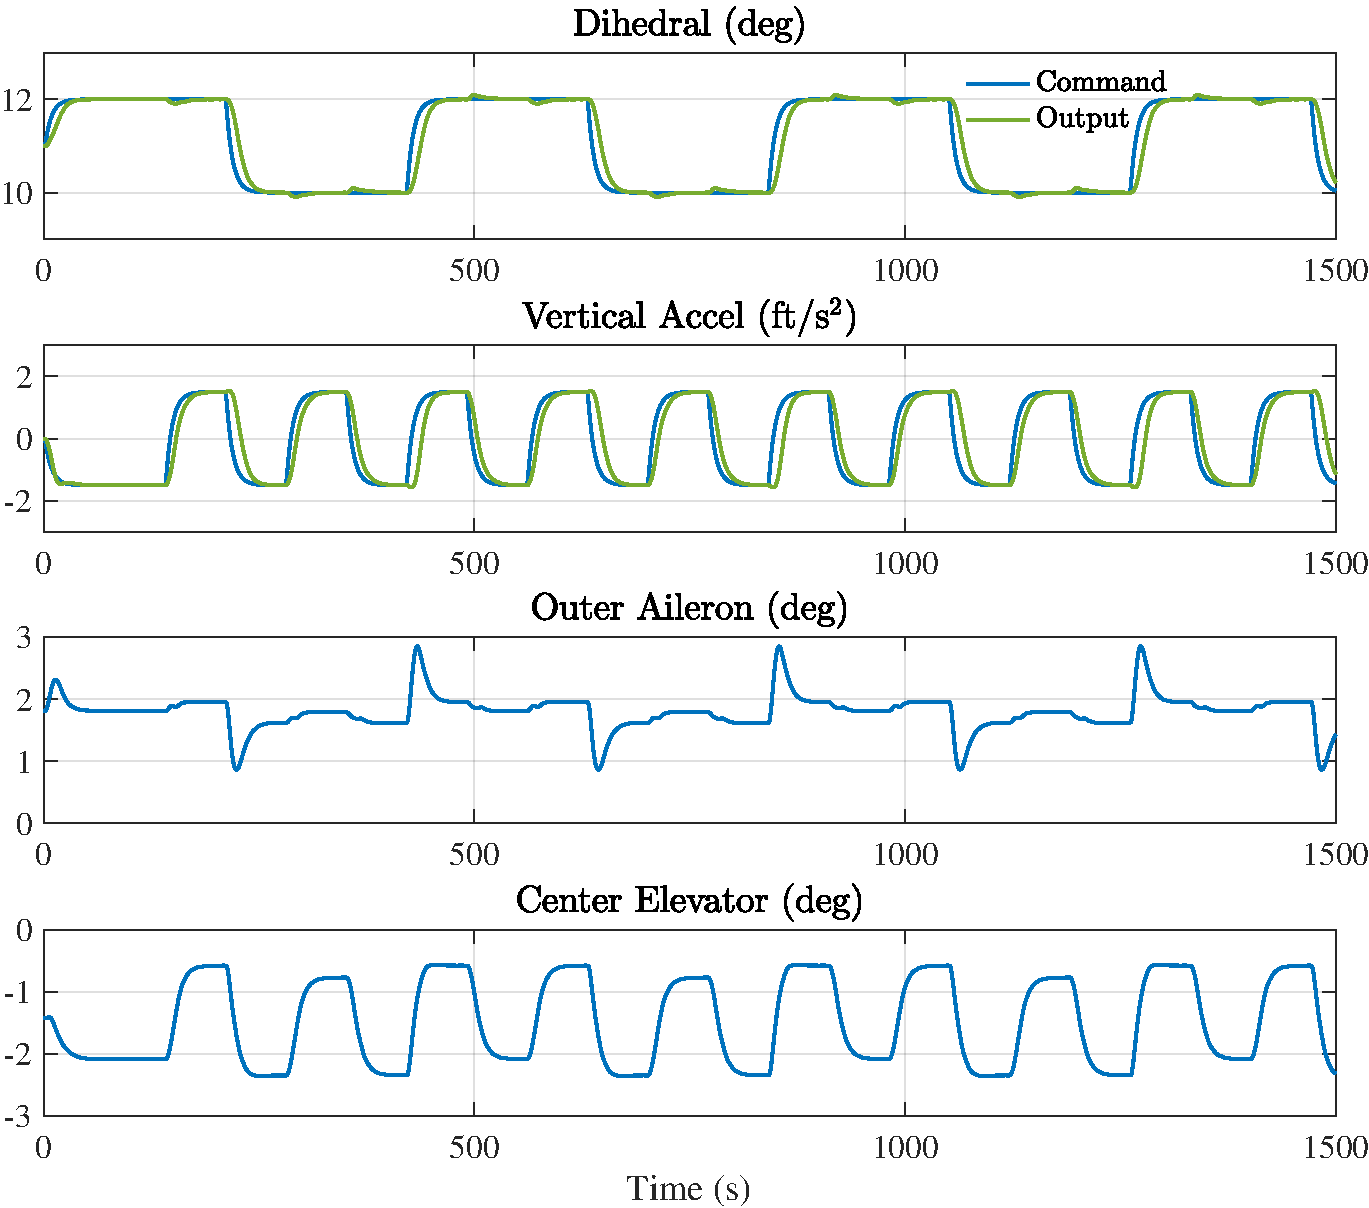
\includegraphics[width=\columnwidth]{nom1.pdf}
	\caption{Nom-1 simulation: RSLQR with no uncertainty in the control model}
	\label{fig:nom1}
\end{figure}

\begin{figure}[htbp]
	\centering
	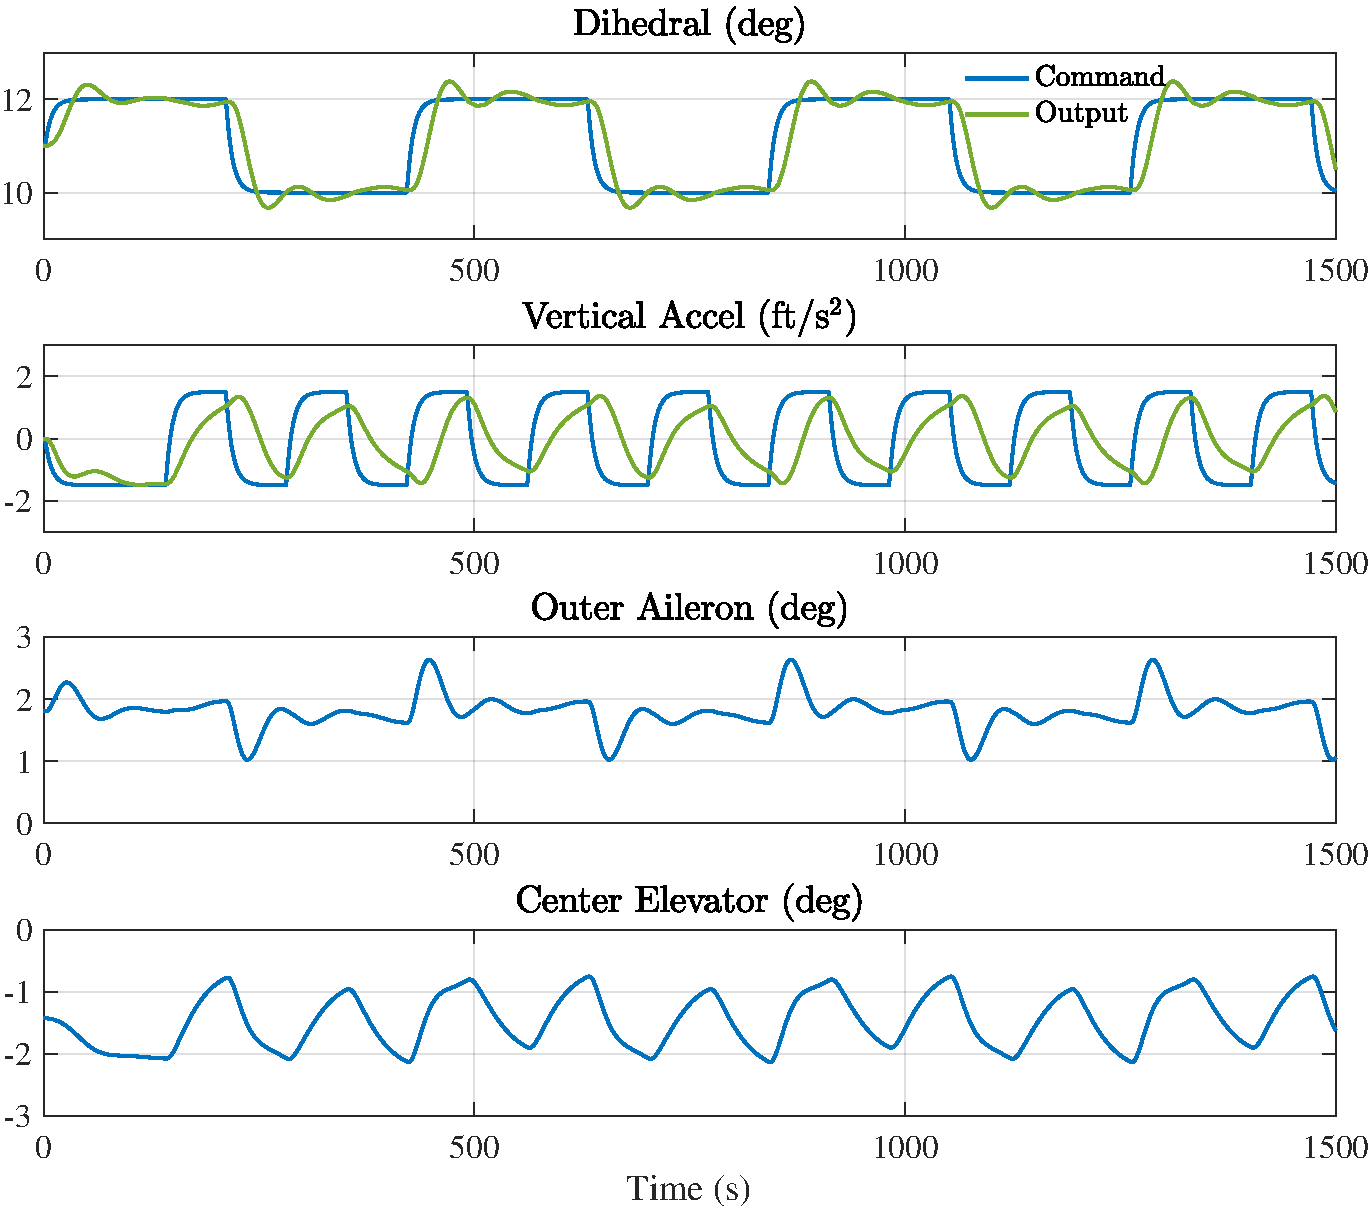
\includegraphics[width=\columnwidth]{nom2.pdf}
	\caption{Nom-2 simulation: RSLQR with uncertainties $\Theta_p$, $\Lambda_p$, and $\Theta_1$}
	\label{fig:nom2}
\end{figure}

\begin{figure}[htbp]
	\centering
	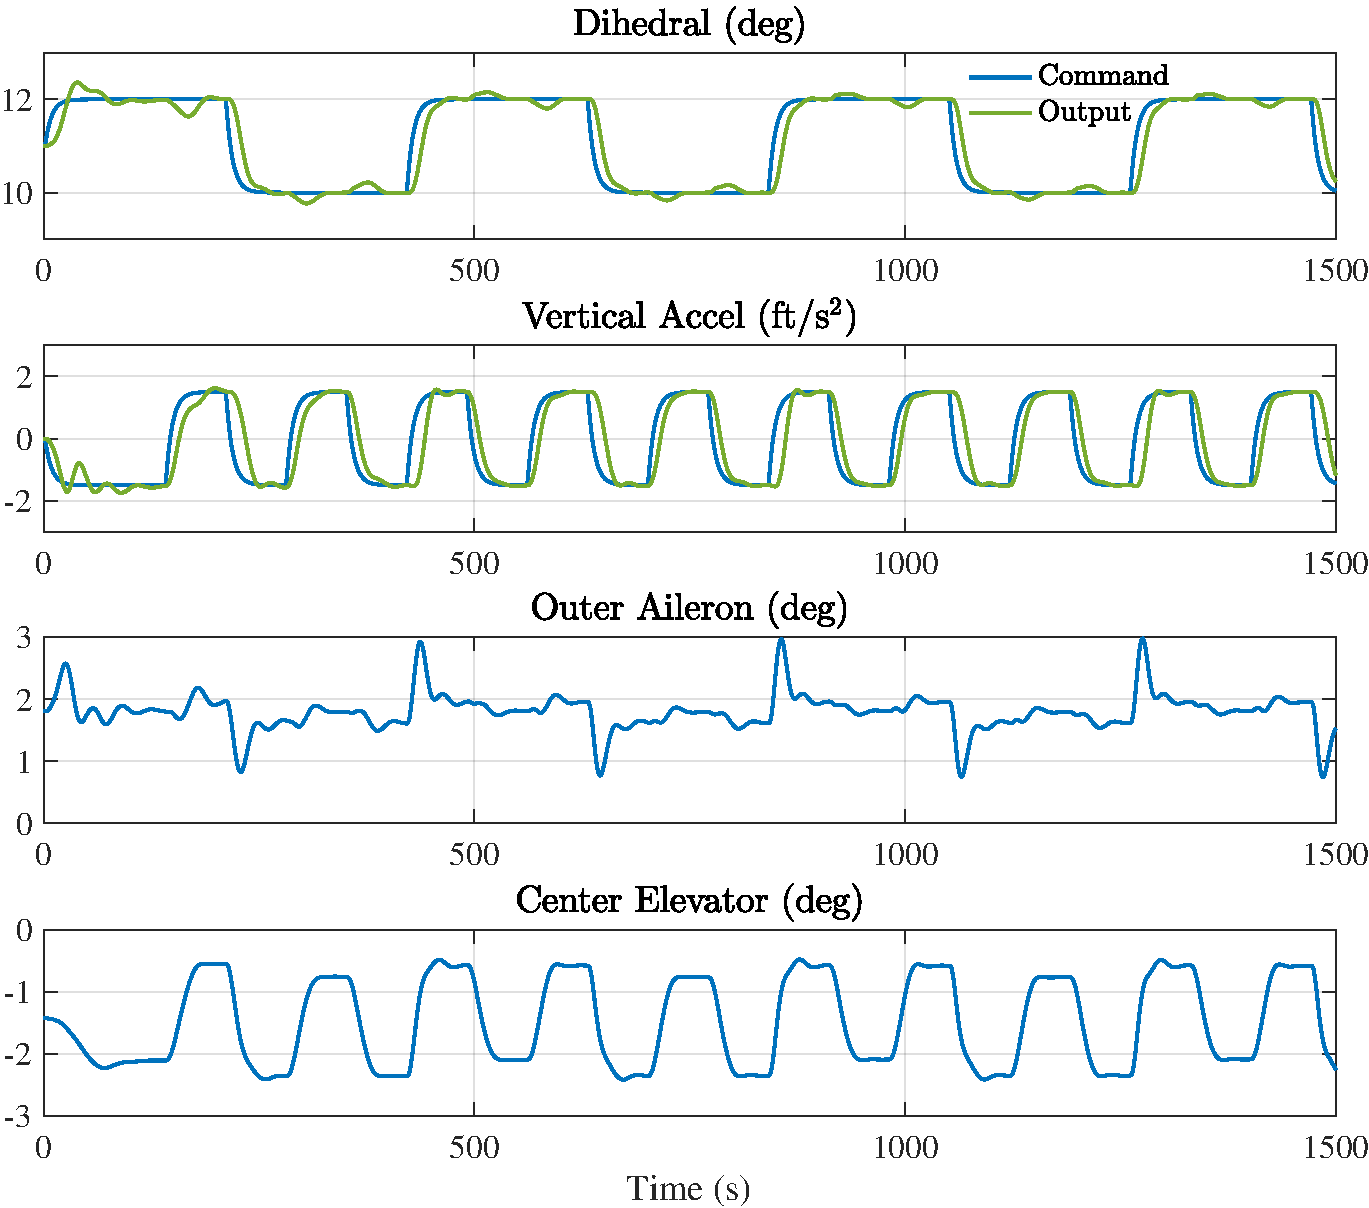
\includegraphics[width=\columnwidth]{nom3.pdf}
	\caption{Nom-3 simulation: RSLQR + MRAC with uncertainties $\Theta_p$, $\Lambda_p$, and $\Theta_1$}
	\label{fig:nom3}
\end{figure}

These simulations, presented in Figs. \ref{fig:nom1}, \ref{fig:nom2}, and \ref{fig:nom3} respectively, show how the MRAC controller with output feedback described in (\ref{eq:rd2-b1a})--(\ref{eq:rd2-adaptation}) is able to recover the desired closed-loop performance with uncertainty in plant and actuator parameters. With the baseline RSLQR controller only, the system suffers degraded command tracking performance in the presence of uncertainty (Fig. \ref{fig:nom2}), especially for vertical acceleration tracking.

We now simulate the introduction of a severe anomaly into the dynamics, causing the actuator dynamics to change suddenly from the uncertain first-order dynamics (\ref{eq:first_order_act}) to the uncertain second-order dynamics (\ref{eq:second_order_act}). The three responses to this anomaly which we will consider are
\begin{description}
	\item[AR-1 (Passive)] The RSLQR+MRAC autopilot retains control without intervention from the remote human supervisor
	\item[AR-2 (Manual)] The human operator takes over manual control of the affected vehicle
	\item[AR-3 (Shared)] Responsibilities are shared between the human pilot and autopilot as described in Section \ref{sec:shared_ctrl}
\end{description}

In these simulations, the vehicle operates in nominal operation with the RSLQR+MRAC control design for $0 \leq t < 600 s$. At $t = 600 s$, the vehicle's actuators change from first-order (\ref{eq:first_order_act}) to second-order (\ref{eq:second_order_act}). Figs. \ref{fig:ar1}--\ref{fig:ar1-err} show the result of a passive response (AR-1) in which the human operator ignores vehicle performance degradation and allows the adaptive controller to continue operating on the plant with severely anomalous dynamics. The closed-loop system loses stability, leading to oscillations in vehicle output and eventual structural failure of the VFA at $t = 960s$, 6 minutes after the introduction of second-order actuator dynamics. It is worth noting the rapid increase in magnitude of the adaptive parameters and the magnitudes of both tracking and measurement output error signals after the introduction of anomalous dynamics. For comparison to a baseline without adaptive control, a passive response using only the RSLQR controller leads to structural failure following the anomaly, at $t = 1240s$.

\begin{figure}[htbp]
	\centering
	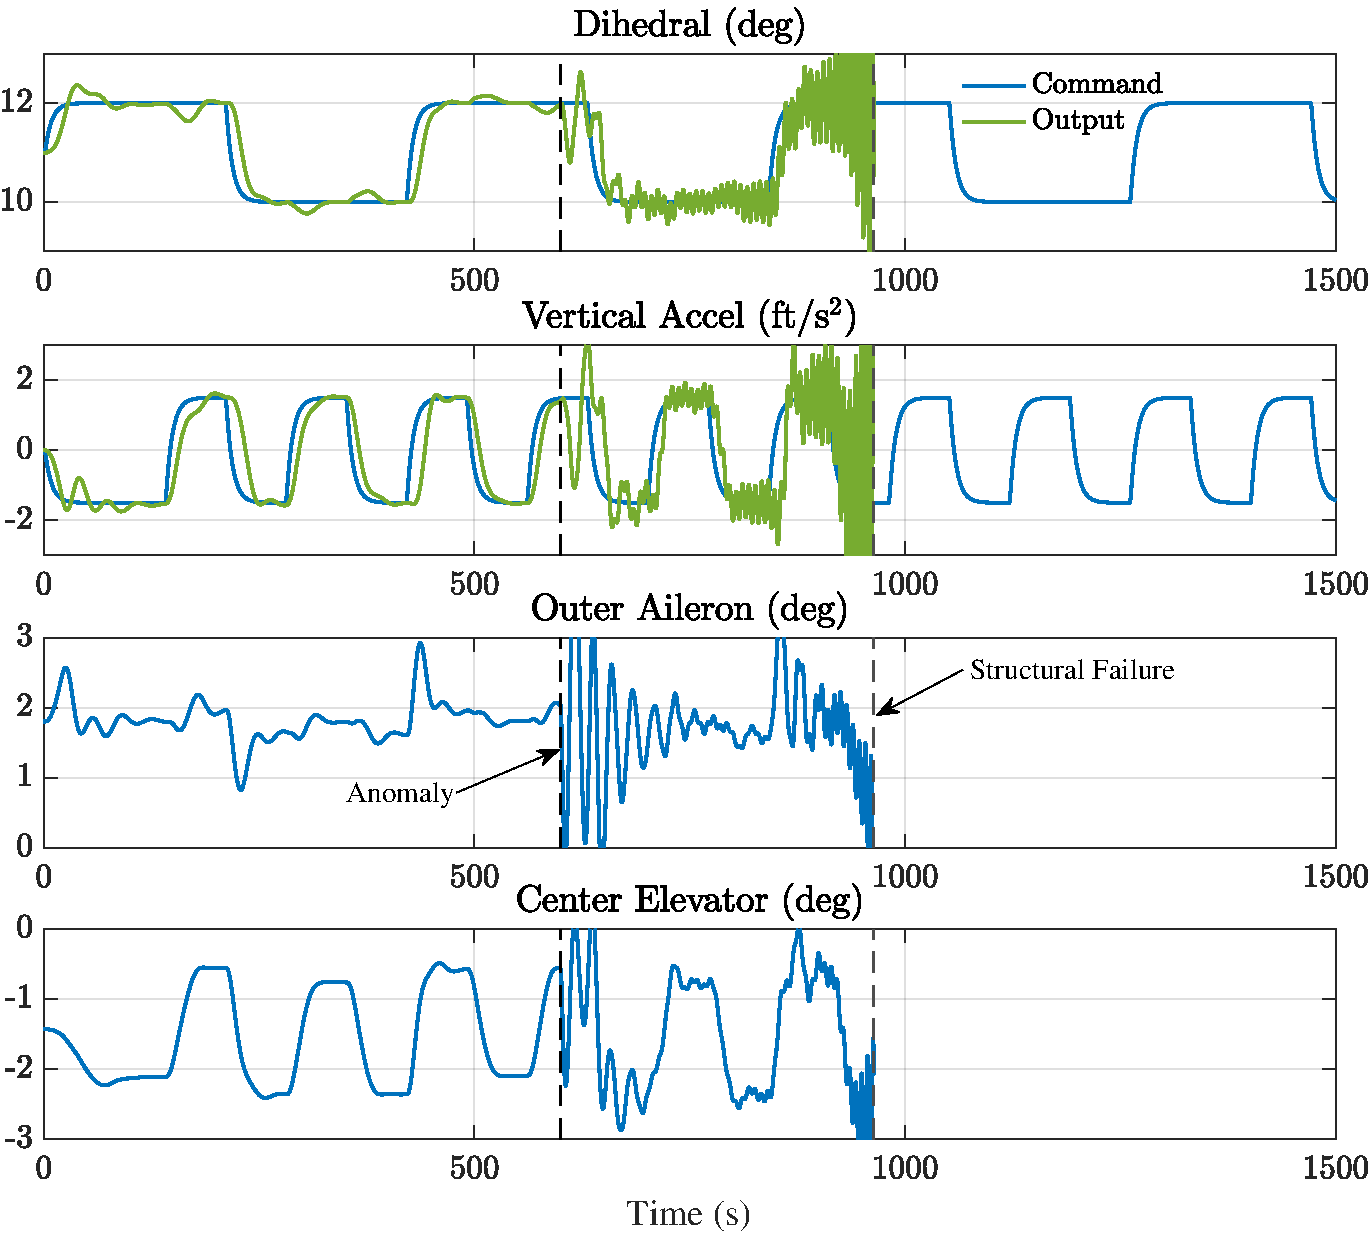
\includegraphics[width=\columnwidth]{ar1.pdf}
	\caption{AR-1 simulation: passive response to dynamical anomaly results in structural failure after 6 minutes}
	\label{fig:ar1}
\end{figure}

\begin{figure}[htbp]
	\centering
	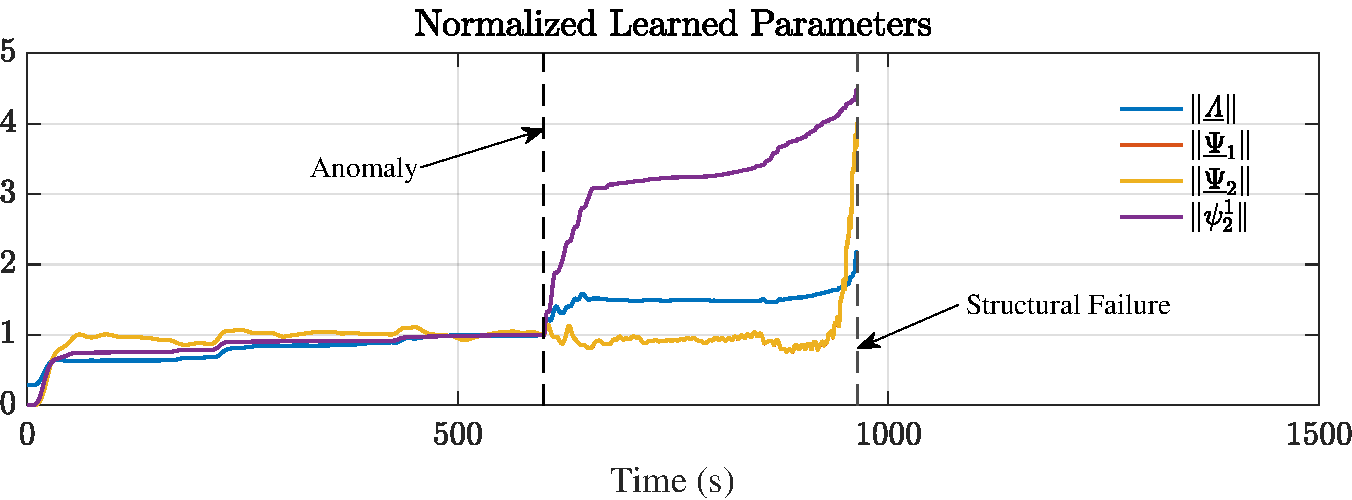
\includegraphics[width=\columnwidth]{ar1-params.pdf}
	\caption{AR-1 simulation: adaptive parameters diverge as controller struggles to adapt to unmodeled dynamics}
	\label{fig:ar1-params}
\end{figure}

\begin{figure}[htbp]
	\centering
	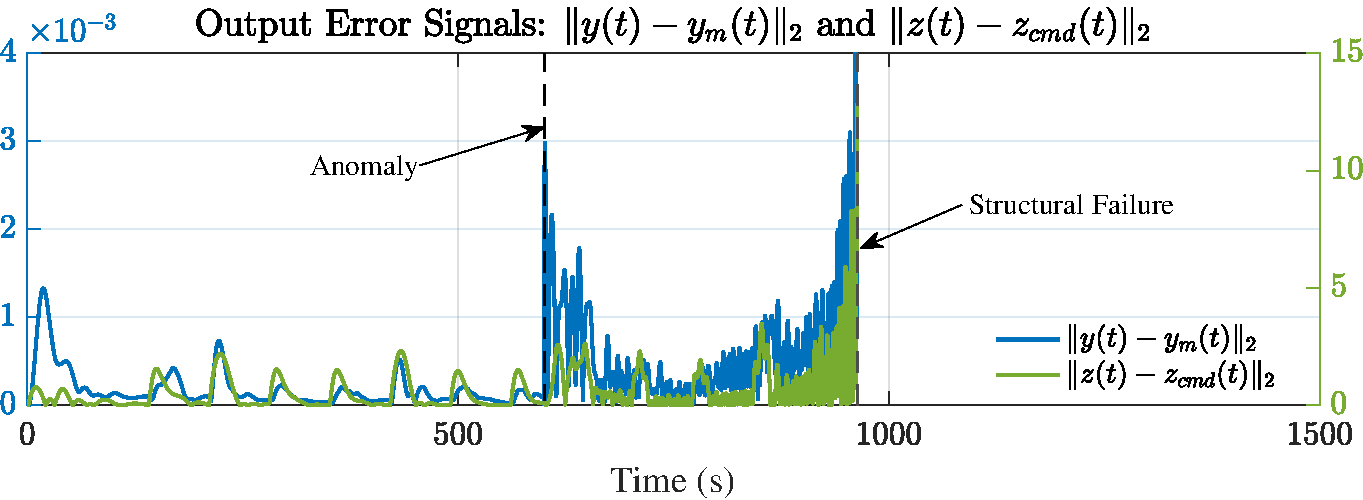
\includegraphics[width=\columnwidth]{ar1-err.pdf}
	\caption{AR-1 simulation: model-following output error and command tracking error grow due to anomalous dynamics}
	\label{fig:ar1-err}
\end{figure}

Numerical simulations of the AR-2 response (purely manual control) are not carried out, as they are not deterministic and require high-fidelity \textit{human-in-the-loop} experiments to characterize. The limitations of such a response -- in which the human operator's role changes suddenly from ``on-the-loop'' to ``in-the-loop'' with unfamiliar dynamics -- are discussed in the earlier sections of this paper.

Results of the AR-3 (shared control) anomaly response simulation are shown in Figs. \ref{fig:ar3-sim}--\ref{fig:ar3-err}. After the anomaly is introduced at $t = 600 s$, the ``nominal'' controller attempts to control the system whose dynamics are not fully accounted for in the control model. Simultaneously in the shared control framework, the human operator notices the anomalous closed-loop control behavior, and via an interface switches the controller to the higher relative degree design (\ref{eq:rd3-b1a})--(\ref{eq:rd3-adaptation-deriv}) at $t = 800 s$, which is the culmination of the human operator's action. For $t \geq 800 s$, the vehicle remains under autonomous control with the ``recovery'' adaptive controller and is able to reestablish nominal command tracking performance. For comparison, the time of structural failure in the passive anomaly response is plotted as a line at $t = 960 s$.

\begin{figure}[htbp]
	\centering
	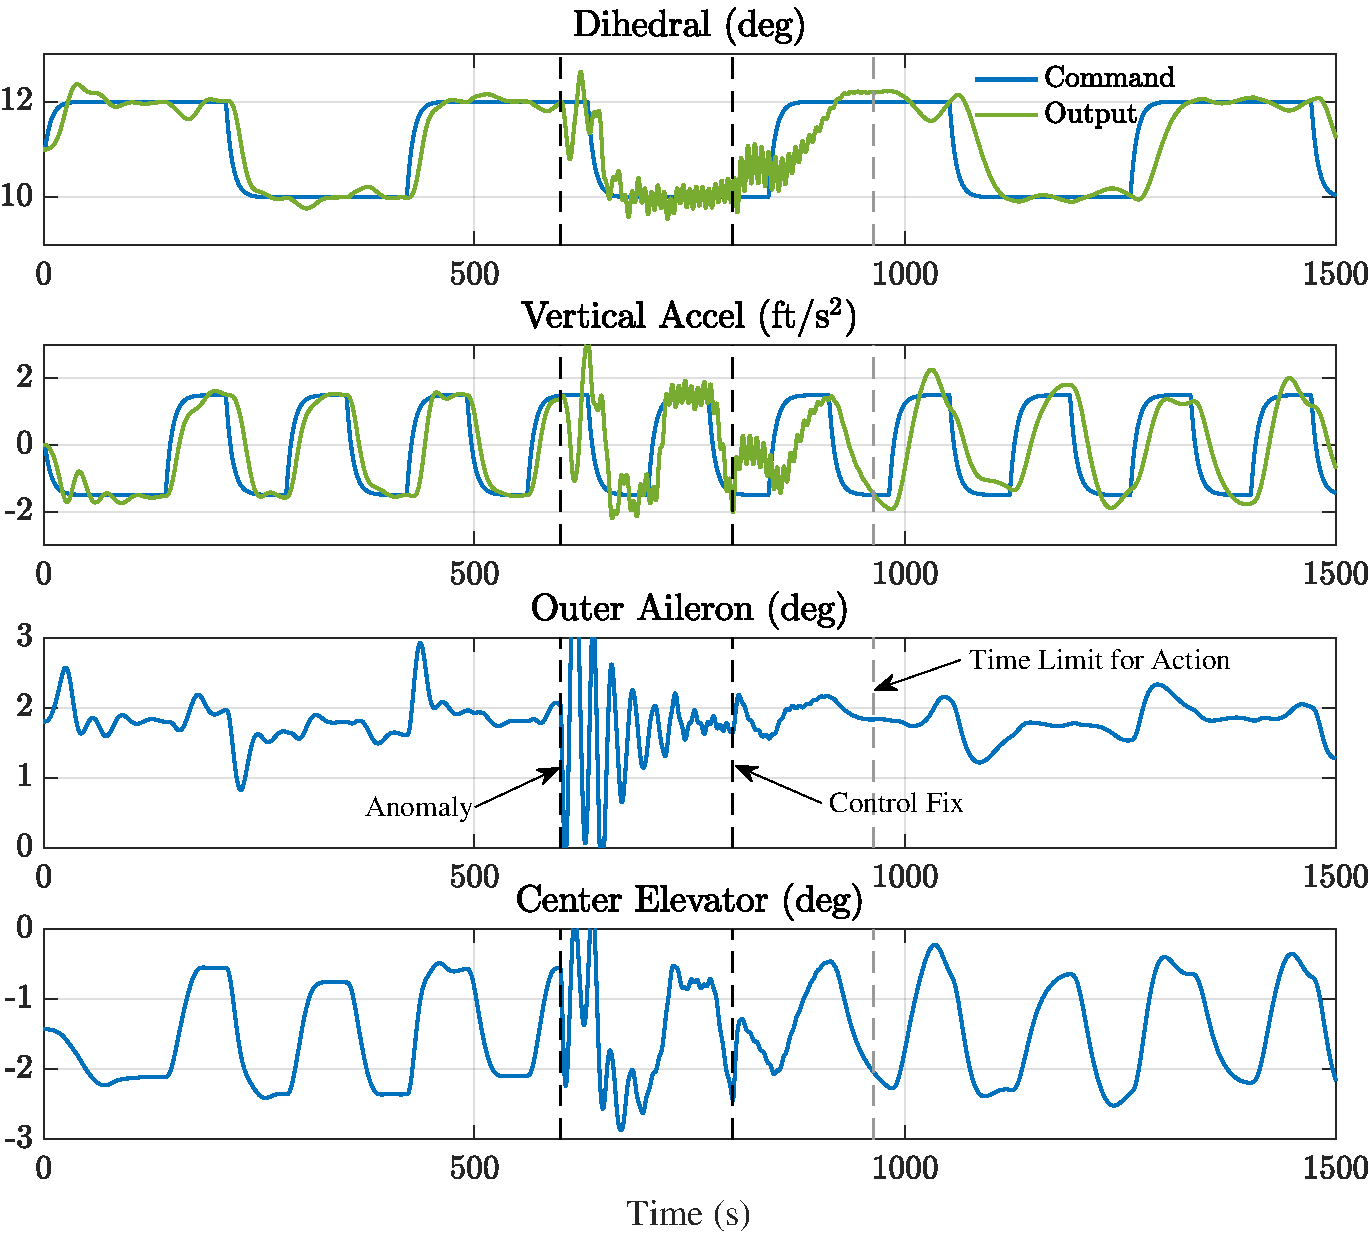
\includegraphics[width=\columnwidth]{ar3.pdf}
	\caption{AR-3 simulation: shared response to the dynamical anomaly results in recovery of vehicle performance}
	\label{fig:ar3-sim}
\end{figure}

\begin{figure}[htbp]
	\centering
	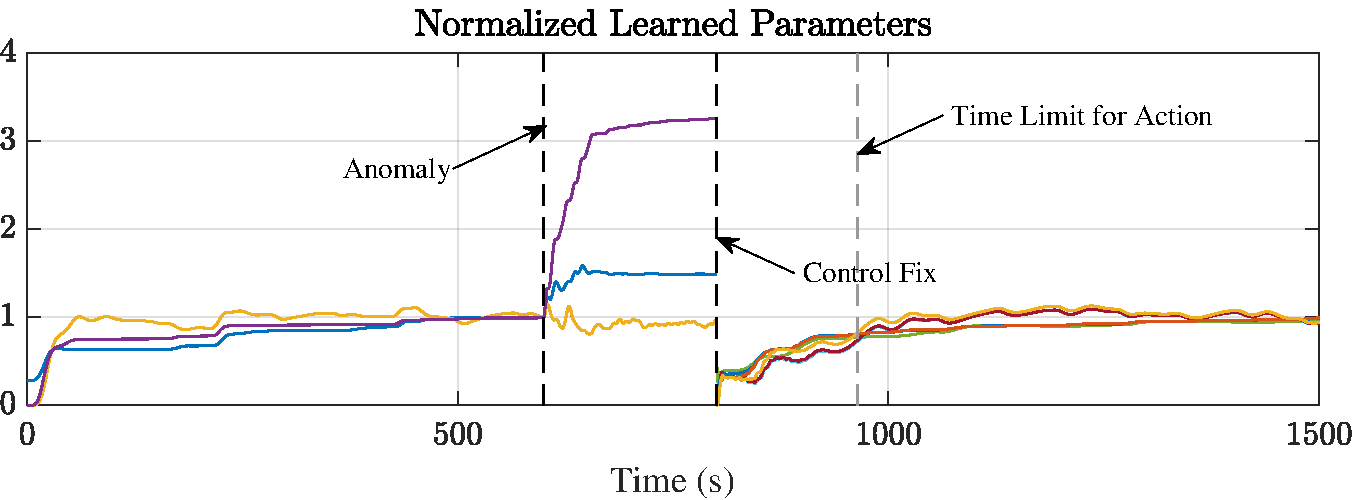
\includegraphics[width=\columnwidth]{ar3-params.pdf}
	\caption{AR-3 simulation: the change in control model at $t = 800 s$ stops the divergence of adaptive parameters}
	\label{fig:ar3-params}
\end{figure}

\begin{figure}[htbp]
	\centering
	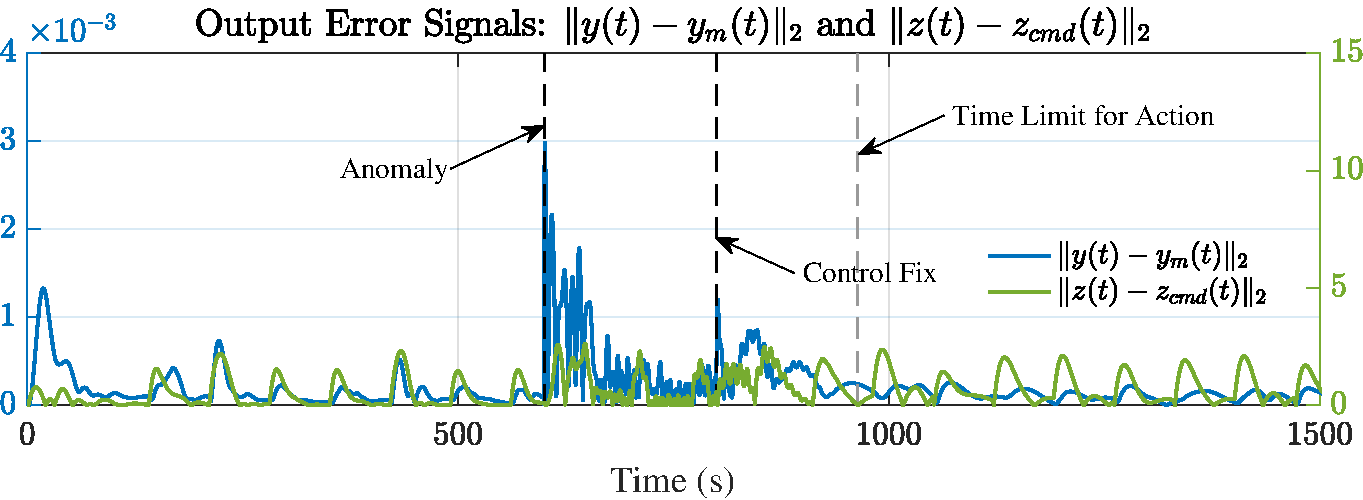
\includegraphics[width=\columnwidth]{ar3-err.pdf}
	\caption{AR-3 simulation: the change in control model at $t = 800 s$ stops the error growth seen after the anomaly}
	\label{fig:ar3-err}
\end{figure}
